%!TEX program = xelatex
%!TEX encoding = UTF-8 Unicode

\documentclass[10pt, twocolumn]{article}
\usepackage[top=1in, bottom=1in, left=1in, right=1in]{geometry}

% ----- ADDITIONAL PACKAGES -----
\usepackage{fontspec,xltxtra,xunicode}
\usepackage{amsmath}
\usepackage[usenames,dvipsnames]{color}
\usepackage[bookmarks, colorlinks, breaklinks, 
  pdftitle={Operations Research: Optimization},
  pdfauthor={Yue Wu},
  pdfcreator={xelatex}
]{hyperref}
\usepackage{multirow}
\usepackage{paralist}

% ----- SETTINGS -----
\setcounter{secnumdepth}{0}
\linespread{1.15}
\setlength\parindent{0pt}
\setlength\parskip{1ex plus 0.2ex minus 0.1ex}
\setlength\emergencystretch{3em}
\hypersetup{linkcolor=blue, citecolor=blue, filecolor=black, urlcolor=MidnightBlue}

% ----- DOCUMENT -----
\begin{document}
\pagestyle{myheadings}
\markright{Yue Wu}

% \section*{Linear Programming}
% \begin{itemize}
% \item \textbf{Assumptions}:
% \begin{itemize}
%   \item Proportionality: the contribution of each activity to the \emph{Objecyive Function} or LHS of each functional \emph{Constraint} is proportional to the level of the activity
%   \item Additivity: every function is proportional to the level of the activity
%   \item Divisibility: the decision variables are allowed to take on any values that satisfy the functional and non-negativity constraints
%   \item Certainty: the value assigned to each parameter is a known constant
% \end{itemize}
% \end{itemize}

% \section*{Simplex Method}
% \begin{itemize}
% \item \textbf{Important Properties}:
% \begin{itemize}
%   \item \#1: single optimal solution $\longrightarrow$ CPF solution; multiple optimal solution $\longrightarrow$ at least two CPF solutions
%   \item \#2: If a CPF solution has no adjacent CPF solutions that are better, then it must be an optimal solution
% \end{itemize}
% \end{itemize}

\section*{Duality \& Sensitivity}
% \[ \boxed{\begin{array}{clrll}
% (P) & max & Z = & \boldsymbol{cx} & \\
% & s.t. & & \boldsymbol{Ax} & \leq \boldsymbol{b} \\
% & & & \boldsymbol{x} & \geq \boldsymbol{0}
% \end{array}} \]
% \[ \boxed{\begin{array}{clrll}
% (D) & min & W = & \boldsymbol{yb} & \\
% & s.t. & & \boldsymbol{yA} & \geq \boldsymbol{c} \\
% & & & \boldsymbol{y} & \geq \boldsymbol{0}
% \end{array}} \]
\[ \boxed{\begin{array}{ccrlll} (P)
& \text{max } & Z = & \sum_{j=1}^nc_jx_j & & \\
& \text{s.t.} & & \sum_{j=1}^na_{ij}x_j & \leq b_i, & \forall i \\
& & & x_j & \geq 0, & \forall j 
\end{array}} \]
\[ \boxed{\begin{array}{ccrlll} (D)
& \text{min } & W = & \sum_{i=1}^mb_iy_i & & \\
& \text{s.t.} & & \sum_{i=1}^ma_{ij}y_i & \geq c_j, & \forall j \\
& & & y_i & \geq 0, & \forall i
\end{array}} \]
\begin{itemize}
\item The Weak Duality Property: $\boldsymbol{cx} \leq \boldsymbol{yb}$
\item The Strong Duality Property: $\boldsymbol{cx}^* = \boldsymbol{yb}^*$
\item Complementary Solution Property: the simplex method simultaneously identifies a CPF solution $\boldsymbol{x}$ and a complementary solution $\boldsymbol{y}$ such that $\boldsymbol{cx} = \boldsymbol{yb}$. ($\boldsymbol{y}$ may be infeasible)
% \item Complementary Optimal Solution Property: 
\item Duality Theorem: (P) \emph{Feasible} and \emph{Bounded} $\longrightarrow$ (D) \emph{Feasible} and \emph{Bounded}; (P) \emph{Feasible} and \emph{Unbounded} $\longrightarrow$ (D) \emph{Infeasible}; (P) \emph{Infeasible} $\longrightarrow$ (D) \emph{Infeasible} or \emph{Unbounded}
\item Shadow Prices $y_i^*$ ($0$ if constrain not tight)
\item Complementary Slackness Conditions: 
\[ \sum\limits_{j=1}^n (c_j-\sum\limits_{i=1}^my_i^*a_{ij})x_j^* + \sum\limits_{i=1}^m y_i^*(\sum\limits_{j=1}^na_{ij}x_j^*-b_i) = 0 \]
For every $j$, either $x_j^*=0$ or $\sum_{i=1}^my_i^*a_{ij}=c_j$; \\
For every $i$, either $y_i^*=0$ or $\sum_{j=1}^na_{ij}x_j^*=b_i$; \\
$x^*$ and $y^*$ are optimal $\Longleftrightarrow$ CSCs hold
\item Complementary Slackness Theorem: Let $\boldsymbol{x}^∗$ be feasible for (P) and $\boldsymbol{y}^∗$ be feasible for (D). Then $\boldsymbol{x}^∗$ and $\boldsymbol{y}^∗$ are optimal if and only if the complementary slackness conditions hold.
\item Universal Transform: 
\begin{table}[h]
\centering
\begin{tabular}{|c|c|c|} \hline
Type     & Primal (max) & Dual (min)   \\ \hline
Sensible & $\leq$       & $y_i \geq 0$ \\
Odd      & $=$          & Unrestricted \\
Bizarre  & $\geq$       & $y_i \leq 0$ \\ \hline
Sensible & $x_j \geq 0$ & $\geq$       \\
Odd      & Unrestricted & $=$          \\
Bizarre  & $x_j \leq 0$ & $\leq$       \\ \hline
\end{tabular}
\end{table} 
\item Sensitivity Analysis:
\begin{figure}[!h]
\centering
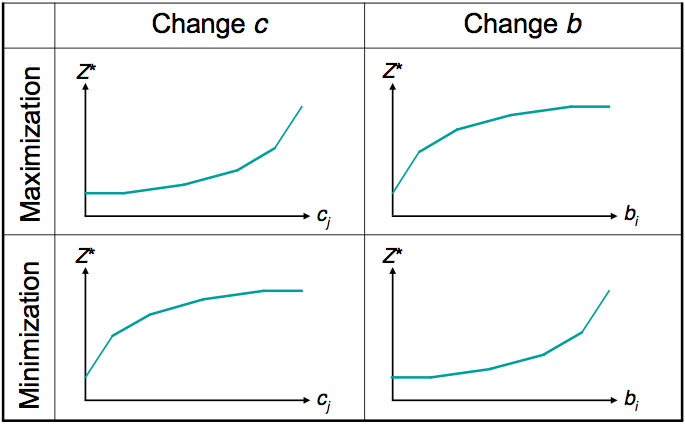
\includegraphics[width=0.45\textwidth]{sensitivity}
\end{figure}
\end{itemize}

\section*{Network Optimization}
\begin{itemize}
\item Network (G), Nodes (V), Arcs (A): $G=(V,A)$
\item Tree: connected network with no cycles
\item Dijkstra's Algorithm for SPP: \input{q4.tex} 
\item Greedy Algorithm for Minimum Spanning Tree Problem: 
\begin{inparaenum}
  \item choose any node and connect its nearest neighbor;
  \item choose node that is closest to the connected nodes until all are connected.
\end{inparaenum}
\item Augmenting Path: path from source to sink that every arc has a \emph{strictly positive residual capacity}.
\item Augmenting Path Algorithm for Maximum Flow Problem: 
\begin{inparaenum}
  \item identify an augmenting path; 
  \item find the minimum residual capacity ($c^*$) of all arcs on the path; 
  \item decrease the capacity of each arc by $c^*$; 
  \item repeat until no augmenting path exists. 
\end{inparaenum}
\item Max-Flow Min-Cut Theorem: for any network, the maximum feasible flow from the source to the sink \emph{equals} the minimum cut value for all cuts in the network. 
\item Integer Solutions Property: for minimum-cost flow problems in which every $b_i$ and $u_{ij}$ have integer values, all basic variables in every basic feasible solution, including every optimal one, also have integer values. 
\item The Min-Cost Flow Problem
\[ \begin{array}{cl}
\text{min } & \sum_{(i,j) \in E}c_{ij}x_{ij} \\
\text{s.t.} & \sum_jx_{ij} - \sum_kx_{ki} = b_i,\ \forall i \\
& l_{ij} \leq x_{ij} \leq u_{ij} \\
& x_{ij} \geq 0,\ \forall (i,j) \ in E
\end{array} \]
\item The Balanced Transportation Problem
\[ \begin{array}{cl}
\text{min } & \sum_{i=1}^m\sum_{j=1}^nc_{ij}x_{ij} \\
\text{s.t.} & \sum_{j=1}^nx_{ij} = a_i,\ \forall i \\
& \sum_{i=1}^mx_{ij}=b_j,\ \forall j \\
& x_{ij} \geq 0,\ \forall i,j
\end{array} \]
\item The Assignment Problem
\[ \begin{array}{cl}
\text{min } & \sum_{i=1}^m\sum_{j=1}^nc_{ij}x_{ij} \\
\text{s.t.} & \sum_{j=1}^nx_{ij} = 1,\ \forall i \\
& \sum_{i=1}^mx_{ij} = 1,\ \forall j \\
& x_{ij} = \{0,1\},\ \forall i,j
\end{array} \]
\item The Maximum Flow Problem
\[ \begin{array}{cl}
\text{min } & v \\
\text{s.t.} & \sum_jx_{ij}-\sum_kx_{ki} = \left\{ \begin{array}{ll}
  v & \text{if } i=s, \\
  -v & \text{if } i=t, \\
  0 & \text{otherwise} \end{array}\right. \\
& 0 \leq x_{ij} \leq u_{ij},\ \forall (i,j) \in E
\end{array} \]
\item The Shortest Path Problem
\[ \begin{array}{cl}
\text{min } & \sum_{(i,j) \in E}c_{ij}x_{ij} \\
\text{s.t.} & \sum_jx_{ij}-\sum_kx_{ki} = \left\{ \begin{array}{ll}
  1 & \text{if } i=s, \\
  -1 & \text{if } i=t, \\
  0 & \text{otherwise} \end{array}\right. \\
& x_{ij} \geq 0,\ \forall (i,j) \in E
\end{array} \]
\end{itemize}

\section*{Integer Programming}
\begin{itemize}
\item LP is easy to solve because there is always an optimal solution that is a CPF solution, which is not necessarily true in IP. 
\item Fixed-Charge Problems: 
\[ \text{min } Z = \sum_{j=1}^n(c_jx_j+k_jy_j) \]
\item Contingent Decisions: 
\[ x_j \leq My_j, \quad\forall j=1,\dots,n \]
in whichi $M$ is a huge number.
\item Either-Or Constraints: 
\[ \text{ConsONE} \leq My,\text{ and }\text{ConsTWO} \leq M(1-y) \]
\item K-out-of-N Constraints:
\[ \sum_ja_{ij}x_{ij} \leq b_i + My_i,\text{ and }\sum_iy_i = N-K \]
\item Constraints with $m$ Possible RHSs: 
\[ \sum_{i=1}^na_ix_i = \sum_{k=1}^md_ky_k,\text{ and }\sum_{k=1}^my_k=1 \]
\item $z = x \texttt{ O\_R } y$: $z \geq x, z \geq y, z \leq x+y$ \\
$z = x \texttt{ AND } y$: $z \leq x, z \leq y, z \geq x+y-1$ 
\item If-Then Constraints: if $f(x)>0$, then $g(x)>0$
\[ -g(x) \leq My, f(x) \leq M(1-y) \]
\item Piecewise Linear Approach ($x=\sum_iz_ib_i$): 
\[ z_1 \leq y_1, z_{k} \leq y_{k-1} + y_{k}, z_n \leq y_{n-1} \]
\[ \sum_{i=1}^{n-1}y_i = 1,\; \sum_{i=1}^nz_i=1,\; y_i\in\{0,1\},\; z_i\geq 0 \]
\item Minimax or Maximin: replace the inner $\text{max}\{\}$ ($\text{min}\{\}$) with a new decision variable $t$, which is an upper (lower) bound for all the terms in $\text{max}\{\}$ ($\text{min}\{\}$).
\item Absolute Values ($\text{min } Z = |x_j|$): $x_j = x_j^+ - x_j^-$ with an objective function $[\text{min } Z = x_j^+ + x_j^-]$, in which $x_j^+, x_j^- \geq 0$. Then, one of $x_j^+$ and $x_j^-$ will be \textbf{zero} in a \emph{minimization} problem.
\item Absolute Values in Constraints: 
\[ \left|\sum a_ix_i\right| \leq b \Rightarrow \sum a_ix_i \leq b \text{ and } -\sum a_ix_i \leq b \]
\item LP Relaxation: $x_i\in\{0,1\} \Rightarrow 0 \leq x_i \leq 1$
\item The LP relaxation of any maximization (min) problem provides an upper (lower) bound on the optimal objective value; The bound attained at child nodes is always less (greater) than or equal to the bound attained at parent nodes.
\item Divide and Conquer: partition the set of feasible solutions into smaller subsets (branching), stop partitioning a particular subset if we can tell it’s no good (fathoming).
\item Branch-and-Bound Algrithm: 
\begin{itemize}
  \item 0. Initialization: set $Z^*=-\infty$; 
  \item 1. Branching: among all unfathomed subproblems, select the one that was created most recently. (If tie, choose the one with larger bound.) Branch to create 2 subproblems setting $x_j =0 \text{ or } 1$; 
  \item 2. Bounding: for each new subproblem solve LP relaxation using simplex method and rounding down optimal $Z$ (assumes objective function coefficients are integer); 
  \item 3. Fathoming: fathom any new subproblem that meets one of the 3 fathoming reasons. If subproblem has integer solution with larger objective value than current incumbent, replace incumbent with it. If there are no remaining (unfathomed) subproblems, stop; the current incumbent is optimal. Otherwise, go to 1.
\end{itemize}
\begin{figure}[!h]
\centering
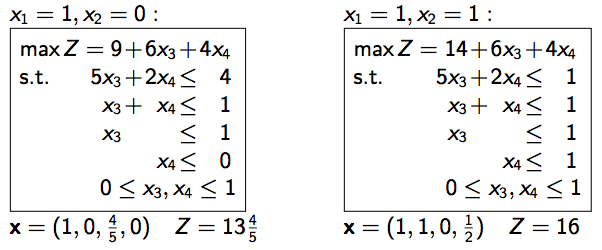
\includegraphics[width=0.5\textwidth]{bab2}
\end{figure}
\begin{figure}[!h]
\centering
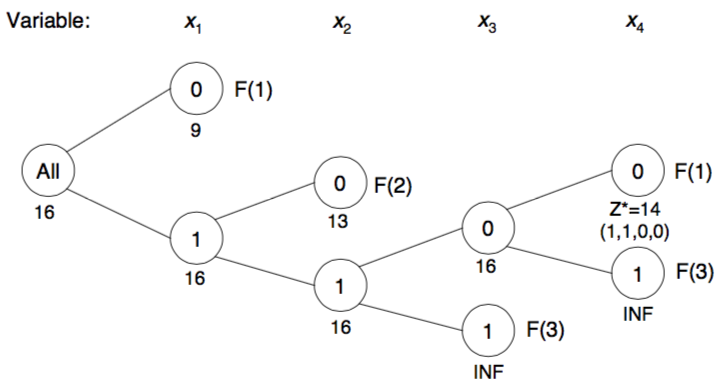
\includegraphics[width=0.5\textwidth]{bab1}
\end{figure}
\item Fathoming Reason: the solution to the LP relaxation is all-integer; OR the optimal objective value for this LP relaxation is less than or equal to the current incumbent value; OR the LP relaxation is infeasible.
\end{itemize}

\section*{Presentations}
\begin{itemize}
\item Type of Industry: supply chain management in micro-electronic industry (IBM Microelectronics Division). 
\item Type of Problem: match assets with demands, to determin which demands it could meet when, and provide manufacturing guidelines.
\item Type of Formulation: linear programming (inventory model) with a traditional material resource planning algorithm and a heuristic matching process based on clues established in the explosion algorithm
\end{itemize}

\section*{Additional Lectures}
\begin{itemize}
\item How to Solve Nonlinear Optimization: use nonlinear solver; take derivatives; numerical search.
\item Some Approaches for Large-Scale LPs: column generation; dantzig wolfe decomposition; constraint generation.
\item $x_{ij}$: pounds produced by reactor $i$ under setting $j$;
$y_{ij}$: $1$ if reactor $i$ is in setting $j$ \textbf{or above}, $0$ otherwise;
$c_{ij}$: unit cost of reactor $i$ in setting $j$;
$P_ij$: the cumulative capacity on reactor $i$ under setting $j$.
\begin{figure}[!h]
\centering
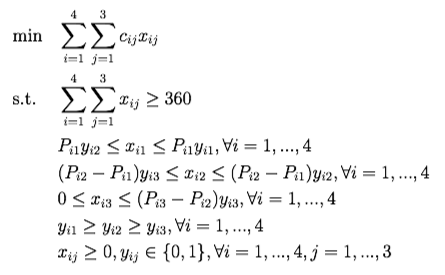
\includegraphics[width=0.5\textwidth]{eg1}
\end{figure}
\item Consider a multi-period production problem over the time period $t = 1,\dots,T$. The relevant data are given below: $d_t=$ demand in period $t$; $c_t=$ fixed cost if anything is produced; $p_t=$ unit production cost; $h_t=$ unit holding cost.
\begin{figure}[!h]
\centering
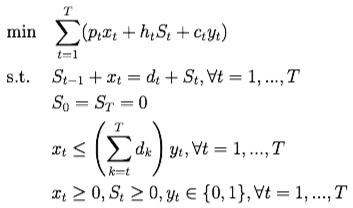
\includegraphics[width=0.5\textwidth]{eg2}
\end{figure}
\begin{figure}[!h]
\centering
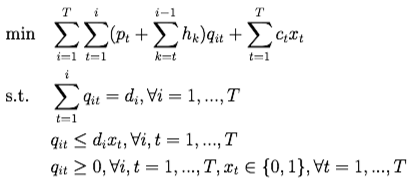
\includegraphics[width=0.5\textwidth]{eg3}
\end{figure}
\item $x_{ij}=$ amount of orders shipped from region $i$ to $j$ using small-parcel; $y_i=$ amount of orders shipped from region $1$ to region $i$ using carrier; $z_i=$ $1$ if MOM shipped orders from region $1$ to region $i$, $0$ otherwise.
\begin{figure}[!h]
\centering
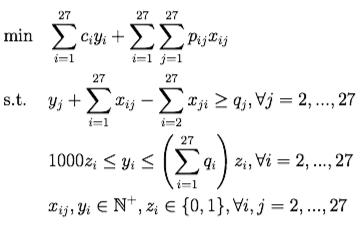
\includegraphics[width=0.5\textwidth]{eg4}
\end{figure}
\item XNOR Gate: 
\[ z_1 \leq 1-x, z_1 \leq 1-y, z_1 \geq 1-x-y \]
\[ z_2 \leq x, x_2 \leq y, z_2 \geq x+y-1  \]
\[ z \geq z_1, z \geq z_2, z \leq z_1+z_2 \]
\end{itemize}
\end{document}